\documentclass[]{abntex2}
\usepackage{lmodern}			% Usa a fonte Latin Modern
\usepackage[T1]{fontenc}		% Selecao de codigos de fonte.
\usepackage[utf8]{inputenc}		% Codificacao do documento (acentuação)
\usepackage{indentfirst}		% Indenta o primeiro parágrafo de cada seção.
\usepackage{nomencl} 			% Lista de simbolos
\usepackage{color}				% Controle das cores
\usepackage{graphicx}			% Inclusão de gráficos
\usepackage{microtype} 			% para melhorias de justificação
\usepackage{amsmath}
\usepackage{float}
% Pacotes adicionais, usados apenas no âmbito do Modelo Canônico do abnteX2
\usepackage{lipsum}				% para geração de dummy text
\usepackage[brazilian,hyperpageref]{backref}% Paginas com as citações na bibl
\usepackage[alf]{abntex2cite}	% Citações padrão ABNT
\usepackage[table]{xcolor}
\usepackage{amssymb}
\usepackage{hyperref}
% Configurações do pacote backref
% Usado sem a opção hyperpageref de backref
\renewcommand{\backrefpagesname}{Citado na(s) página(s):~}
% Texto padrão antes do número das páginas
\renewcommand{\backref}{}
% Define os textos da citação
\renewcommand*{\backrefalt}[4]{
	\ifcase #1 %
		Nenhuma citação no texto.%
	\or
		Citado na página #2.%
	\else
		Citado #1 vezes nas páginas #2.%
	\fi}%

% ---
% Informações de dados para CAPA e FOLHA DE ROSTO
% ---
\titulo{Lista 3 - Fundamentos em Redes Neurais e \\Aprendizagem Estatística}
\autor{Lorran de Araújo Durães Soares\thanks{lorranspbr@gmail.com}}
\local{Petrópolis - RJ - Brasil}
\data{2024}
% ---

% ---
% Configurações de aparência do PDF final
% alterando o aspecto da cor azul
\definecolor{blue}{RGB}{41,5,195}

% ---
% compila o indice
% ---
\makeindex
% ---

% ---
% Altera as margens padrões
\setlrmarginsandblock{3cm}{3cm}{*}
\setulmarginsandblock{3cm}{3cm}{*}
\checkandfixthelayout
% O tamanho do parágrafo é dado por:
\setlength{\parindent}{1.3cm}
% Controle do espaçamento entre um parágrafo e outro:
\setlength{\parskip}{0.2cm}  % tente também \onelineskip
% Espaçamento simples
\SingleSpacing


\begin{document}

% Retira espaço extra obsoleto entre as frases.
\frenchspacing 

\maketitle

\section*{\textbf{Introdução}}
\addcontentsline{toc}{section}{Introdução}

Este documento refere-se à elaboração da terceira lista de exercícios da disciplina de Fundamentos de Redes Neurais e Aprendizagem Estatística, promovida pelo Laboratório Nacional de Computação Científica (LNCC) sob a orientação do professor Gilson Antonio Giraldi. A lista consiste em três questões, que serão apresentadas neste formato de artigo, detalhando o passo a passo necessário para a resolução e implementação de cada uma delas. Todas as questões foram implementadas na linguagem Python, utilizando notebooks do tipo iPynb e empregando bibliotecas como \texttt{Keras} \cite{keras}, \texttt{Pandas} \cite{pandas}, \texttt{Matplotlib} \cite{matplotlib}, \texttt{Numpy} \cite{numpy}, \texttt{Scikit-learn} \cite{scikit-learn}, \texttt{OpenCV} \cite{opencv}, \texttt{Seaborn} \cite{seaborn} e \texttt{PIL} \cite{pillow}. As implementações de todas as questões serão disponibilizadas ao final da explicação de cada uma delas neste documento.

Para a realização de todas as questões, foi utilizada a base de imagens CIFAR-10, fornecida pelo \texttt{Keras}. Esse conjunto de dados é composto por 60.000 imagens coloridas de dimensão 32x32 pixels, distribuídas em 10 classes. Entretanto, foi realizada uma filtragem para trabalhar com a classificação de apenas duas classes de imagens, aviões e carros, reduzindo então o conjunto para 12.000 imagens. Algumas dessas imagens são ilustradas na Figura \ref{fig:amostra}. Além disso, devido a limitações de hardware, nos exercícios 1 e 3, foram utilizados apenas 1.200 das 12.000 imagens.

\begin{figure}[H]
    \centering 
    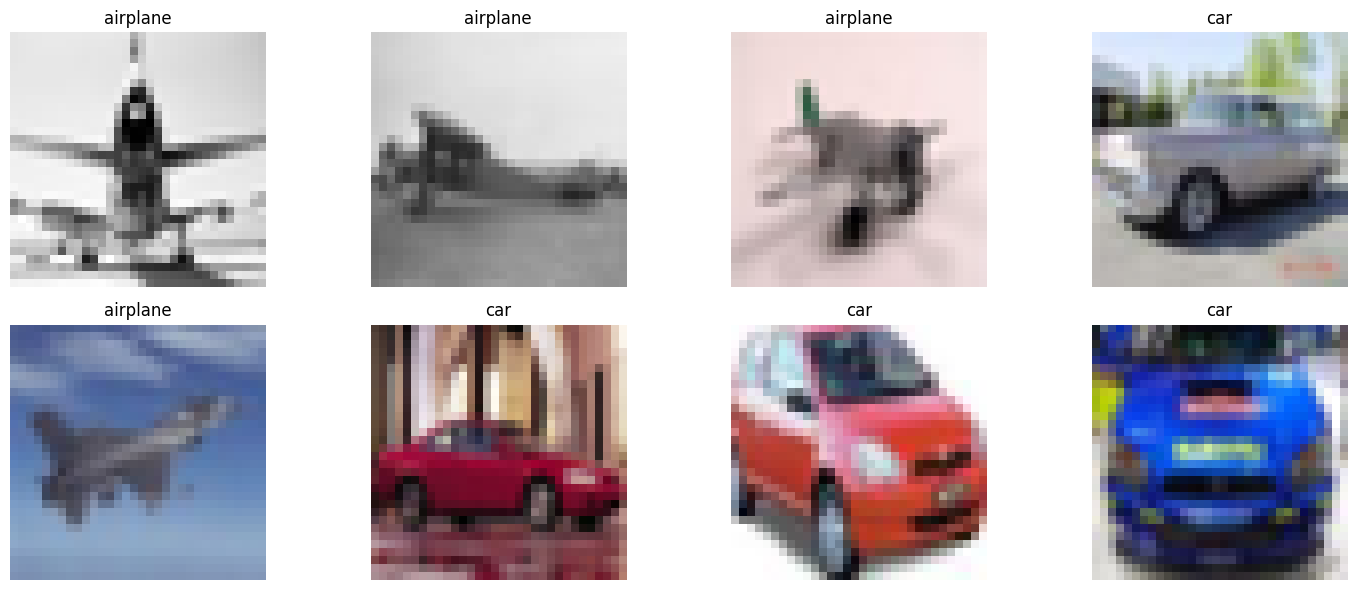
\includegraphics[width=0.9\textwidth]{imgs/introduction/amostra.png}
    \caption{Amostra do banco de imagens}
    \label{fig:amostra} % cria um rótulo para referência no texto
\end{figure}


Esse banco de imagens foi importado da classe \texttt{datasets.cifar10} da biblioteca \texttt{Keras} através da função \texttt{load\_data()}. A escolha de usar um mesmo banco de dados em todas as questões se objetivou em realizar uma comparação entre as diferentes estratégias de classificação que cada exercício pede.


%=================================================================================================
%=================================================================================================
%=================================================================================================
%=================================================================================================
%=================================================================================================
%=================================================================================================
%=================================================================================================
%=================================================================================================
%=================================================================================================
%=================================================================================================
%=================================================================================================


\section*{\textbf{Pré-processamento}}
\addcontentsline{toc}{section}{Pré-processamento}

Para a realização dos exercícios 1 e 3, foi realizado um pré-processamento dos dados, necessário para a execução das operações nessas questões e para obter uma melhor acurácia nos resultados.

As seguintes operações foram realizadas:

\begin{itemize}
    \item Conversão para escala de cinza: realizada através da biblioteca \texttt{OpenCV}, utilizando a função \texttt{cvtColor};
    \item Vetorização das imagens: realizada através do método \texttt{reshape} da biblioteca \texttt{Numpy};
    \item Normalização das features: realizada através da ferramenta \texttt{StandardScaler} da biblioteca \texttt{Scikit-Learn}. O \texttt{StandardScaler} ajusta cada feature do conjunto de dados de acordo com a fórmula:
    
    \[
    z = \frac{x - \mu}{\sigma}
    \]
    
    Onde:
    \begin{itemize}
        \item \( x \) é o valor original da feature.
        \item \( \mu \) é a média dos valores da feature.
        \item \( \sigma \) é o desvio padrão da feature.
    \end{itemize}
    
\end{itemize}

Após isso, através da ferramenta \texttt{train\_test\_split} da biblioteca \texttt{Scikit-Learn}, o conjunto de dados foi separado com proporção de 70\% para treinamento e 30\% para teste. Além disso, com o intuito de realizar a comparação sob o mesmo conjunto de dados para todas as questões, foi selecionada a opção \texttt{random\_state} = 42 na função utilizada para a separação dos dados, fixando a semente de sorteio dos dados. Na implementação de cada uma das questões foi realizado o cálculo da quantidade de imagens de cada classe no conjunto de treinamento, com o intuito de observar possíveis desbalanceamentos de dados. Como mostra a Figura \ref{fig:distri}, as duas classes tinham números de dados iguais, não sendo necessário, portanto, a exclusão ou adição de novos dados no conjunto de treinamento para a realização dos exercícios.

\begin{figure}[H]
    \centering 
    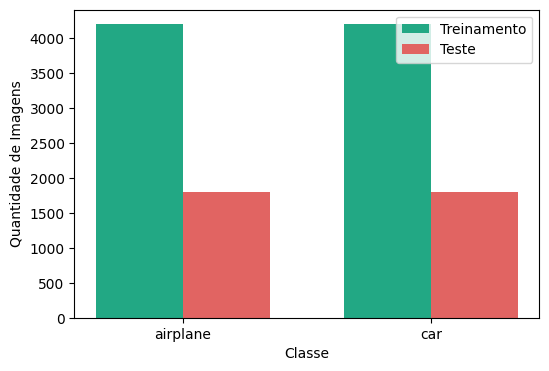
\includegraphics[width=0.5\textwidth]{imgs/introduction/distri.png}
    \caption{Histograma da quantidade de imagens por classe para treinamento e teste}
    \label{fig:distri} % cria um rótulo para referência no texto
\end{figure}


%=================================================================================================
%=================================================================================================
%=================================================================================================
%=================================================================================================
%=================================================================================================
%=================================================================================================
%=================================================================================================
%=================================================================================================
%=================================================================================================
%=================================================================================================
%=================================================================================================


\section*{\textbf{Questão 1}}
\addcontentsline{toc}{section}{Questão 1}

\textit{\begin{enumerate}
    \item Considere um banco de dados de imagens e um problema de classificação. Aplique validação cruzada leave-one-out multi-fold explicada na seção 8.5 de \cite{book}, com $K = 4$, e SVM como segue:
    \begin{enumerate}
        \item SVM Linear não separável com espaço de características obtido através do KPCA.
        \item SVM Kernel não separável com espaço de características obtido através do PCA.
        \item Compare os resultados dos itens (a) e (b).
    \end{enumerate}
\end{enumerate}
}

Para a realização deste exercício, especificamente para o proposto na letra (a), foi inicialmente realizado o cálculo do KPCA através da biblioteca \texttt{Scikit-Learn} com a função \texttt{KernelPCA}. Foi escolhido um kernel polinomial para o cálculo da matriz KPCA com todas as componentes, para posteriormente selecionar as principais componentes. A projeção do conjunto nas duas primeiras componentes do KPCA está ilustrada na Figura \ref{fig:KPCA}.

\begin{figure}[H]
    \centering 
    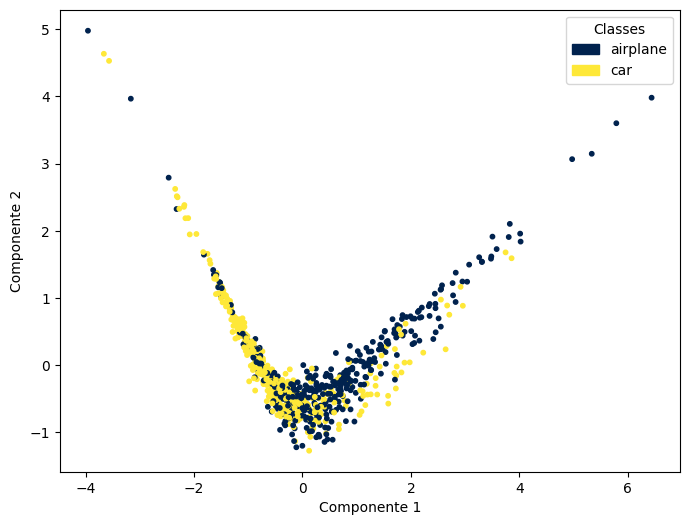
\includegraphics[width=0.5\textwidth]{imgs/ex1/KPCA.png}
    \caption{Projeção do conjunto de treinamento na base obtida pelo KPCA}
    \label{fig:KPCA} % cria um rótulo para referência no texto
\end{figure}

Após o cálculo, foi plotado o gráfico da {\color{red}variância explicada cumulativa}, mostrado na Figura \ref{fig:vari_kpca}. Para a escolha das componentes principais, utilizando a biblioteca \texttt{Numpy} com a função \texttt{argmax}, foi calculado o número de componentes necessário para explicar no mínimo 95\% da variância dos dados, resultando em 435 componentes. A partir disso, a matriz KPCA calculada anteriormente foi reduzida para este número de componentes.

\begin{figure}[H]
    \centering 
    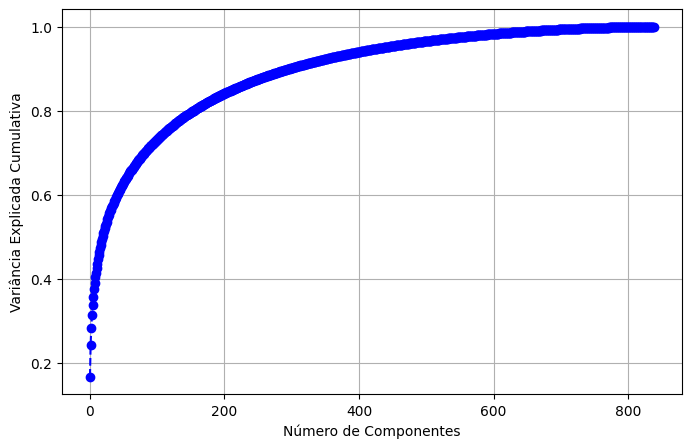
\includegraphics[width=0.6\textwidth]{imgs/ex1/vari_kpca.png}
    \caption{Gráfico da variância explicada cumulativa por componentes KPCA}
    \label{fig:vari_kpca} % cria um rótulo para referência no texto
\end{figure}

Utilizando então um \texttt{K-fold} = 4 {\color{red}(explicar melhor)}, através da função \texttt{SVC} da biblioteca \texttt{Scikit-Learn}, foi construído o SVM, com o objetivo de performar a classificação dos dados. O resultado da acurácia para cada fold sobre os conjuntos de validação e de testes está presente na Tabela \ref{tab:kpca_svm}. Em média, pode-se observar que o classificador construído obteve maior acurácia no conjunto de testes do que no de validação.

\begin{table}[H]
    \centering
    \begin{tabular}{|c|c|c|c|c|c|}
    \hline
    \rowcolor[HTML]{C0C0C0} 
    Conjunto                          & Fold 1 & Fold 2 & Fold 3 & Fold 4 & Média  \\ \hline
    \cellcolor[HTML]{C0C0C0}Validação & 0.60   & 0.69   & 0.57   & 0.60   & 0.615  \\ \hline
    \cellcolor[HTML]{C0C0C0}Teste     & 0.72   & 0.74   & 0.71   & 0.72   & 0.7225 \\ \hline
    \end{tabular}
    \caption{Acurácia da classificação do SVM Linear com o KPCA}
    \label{tab:kpca_svm}
\end{table}

A fim de promover uma visualização gráfica para exemplificar como seria o plano de separação para apenas as duas primeiras componentes obtidas pelo cálculo do KPCA, foi realizado o treinamento de um novo SVM linear, obtendo a reta de separação mostrada na Figura \ref{fig:kpca_reta}, juntamente com a projeção do conjunto de treinamento nessas duas direções. Neste caso, a acurácia média obtida no conjunto de testes foi de 61\%, inferior à de 72\% obtida anteriormente com todas as componentes principais, evidenciando que a redução de dimensionalidade para apenas duas componentes principais impactou na redução da performance do classificador.

\begin{figure}
    \centering 
    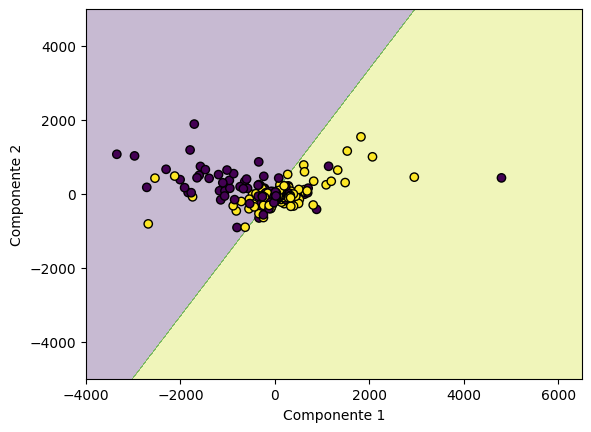
\includegraphics[width=0.6\textwidth]{imgs/ex1/kpca_reta.png}
    \caption{Reta de decisão do SVM Linear com KPCA}
    \label{fig:kpca_reta} % cria um rótulo para referência no texto
\end{figure}

\newpage

De maneira parecida como feito anteriormente para o item a, agora especificamente referente ao item (b), foi inicialmente realizado o cálculo do PCA utilizando a biblioteca \texttt{Scikit-Learn} com a função \texttt{PCA}. Neste primeiro passo, foram calculadas todas as componentes principais, permitindo posteriormente a seleção das mais relevantes. A projeção do conjunto de dados na base PCA está representada na Figura \ref{fig:PCA}.

\begin{figure}[H]
    \centering 
    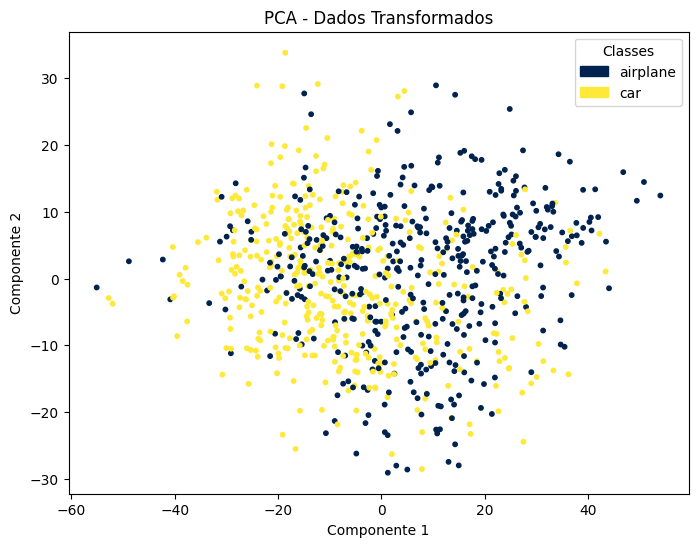
\includegraphics[width=0.5\textwidth]{imgs/ex1/PCA.png}
    \caption{Projeção do conjunto de treinamento na base PCA}
    \label{fig:PCA} % cria um rótulo para referência no texto
\end{figure}

Após o cálculo das componentes principais, foi gerado o gráfico da variância explicada cumulativa, fornecido pelo próprio cálculo do PCA através do método \texttt{explained\_variance\_ratio\_}. O  resultado obtido está ilustrado na Figura \ref{fig:vari_pca}. Para identificar as componentes principais, foi utilizada a função \texttt{argmax} da biblioteca \texttt{Numpy}, determinando o número de componentes necessário para explicar pelo menos 95\% da variância dos dados, resultando em 123 componentes. Com isso, a matriz PCA foi reduzida para conter apenas essas componentes.

\begin{figure}[H]
    \centering 
    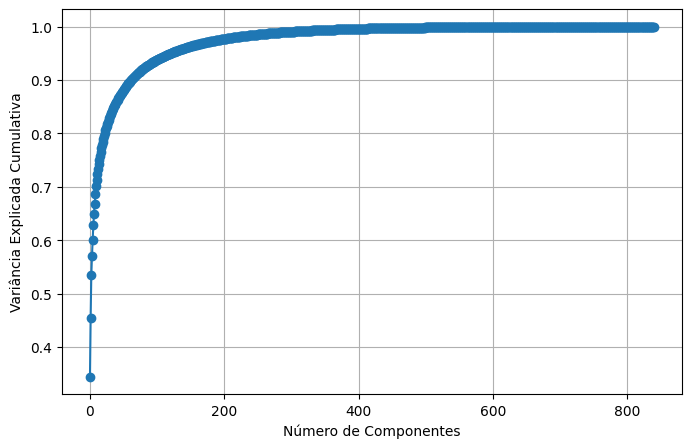
\includegraphics[width=0.5\textwidth]{imgs/ex1/vari_pca.png}
    \caption{Gráfico da variância explicada cumulativa para as componentes do PCA}
    \label{fig:vari_pca} % cria um rótulo para referência no texto
\end{figure}

Em seguida, foi aplicado um \texttt{K-fold} com valor 4 {\color{red}(explicar melhor)}, e, utilizando a função \texttt{SVC} da biblioteca \texttt{Scikit-Learn}, foi construído um SVM com kernel polinomial, com o objetivo de performar a classificação dos dados, obtendo as acurácias mostradas na Tabela \ref{tab:pca_svm} para os conjuntos de validação e de teste.

\begin{table}[H]
    \centering
    \begin{tabular}{|c|c|c|c|c|c|}
    \hline
    \rowcolor[HTML]{C0C0C0} 
    Conjunto                          & Fold 1 & Fold 2 & Fold 3 & Fold 4 & Média  \\ \hline
    \cellcolor[HTML]{C0C0C0}Validação & 0.60   & 0.69   & 0.57   & 0.60   & 0.615  \\ \hline
    \cellcolor[HTML]{C0C0C0}Teste     & 0.72   & 0.74   & 0.71   & 0.72   & 0.7225 \\ \hline
    \end{tabular}
    \caption{Acurácia da classificação do SVM Polinomial com o PCA}
    \label{tab:pca_svm}
\end{table}

Com o intuito de visualizar o plano de separação utilizando apenas as duas primeiras componentes obtidas pelo PCA, foi treinado um novo SVM polinomial considerando apenas as duas primeiras componentes principais obtidas pelo PCA, e a curva de separação foi gerada, como mostrado na Figura \ref{fig:pca_reta}. Essa figura também mostra a projeção do conjunto de treinamento nas duas primeiras direções principais. Nesse cenário, a acurácia média alcançada foi de 61\%.

\begin{figure}[H]
    \centering 
    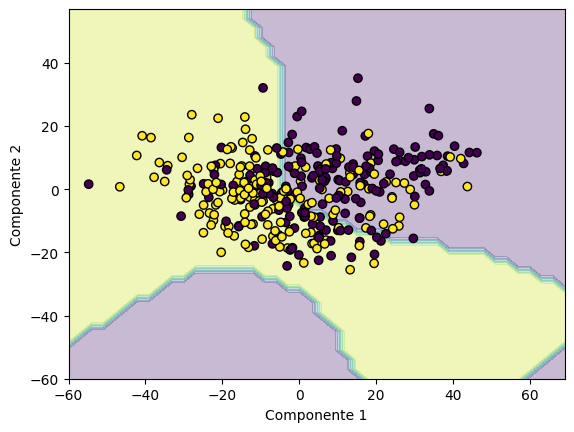
\includegraphics[width=0.5\textwidth]{imgs/ex1/pca_reta.png}
    \caption{Curva de decisão do SVM Polinomial com PCA}
    \label{fig:pca_reta} % cria um rótulo para referência no texto
\end{figure}

{\color{red}Falta falar da comparação entre elas.}


%=================================================================================================
%=================================================================================================
%=================================================================================================
%=================================================================================================
%=================================================================================================
%=================================================================================================
%=================================================================================================
%=================================================================================================
%=================================================================================================
%=================================================================================================
%=================================================================================================



\section*{\textbf{Questão 2}}
\addcontentsline{toc}{section}{Questão 2}

\textit{2. Considere um banco de dados e um problema de classificação. Aplique a validação cruzada multi-fold leave-one-out explicada na seção 8.5 de \cite{book}, com $K = 5$, para um modelo de CNN. Utilize as facilidades disponíveis em bibliotecas para a implementação de redes neurais, como Keras, TensorFlow, etc.}

\textit{\begin{enumerate}
    \item[(a)] Mostre a representação gráfica da evolução das etapas de treinamento e validação (ver Figura 8.8 da monografia do curso).
    \item[(b)] Realize uma análise estatística do desempenho (seção 8.6) dos cinco modelos aplicados sobre a $\mathbb{D}_{te}$.
\end{enumerate}}


Para a realização deste exercício, foram utilizadas todas as 12.000 imagens da base de dados CIFAR-10 referentes às classes aviões e carros, com o objetivo ter mais dados para o treinamento. 

A rede CNN construída para a realização deste exercício teve arquitetura inspirada na rede LeNet-5, desenvolvida para a classificação de imagens, como dígitos numéricos \cite{lecun1998gradient}. Como mostra a tabela \ref{tab:arquiCNN}, a rede construída possui 3 camadas convulucionais, 2 de pooling, 1 de vetorização e 2 camadas MLP densas para a realização da classificação.

Além disso, para a determinação dos hiperparâmetros do otimizador, foi realizado um \textit{grid search} por meio da biblioteca \texttt{Scikit-Learn} utilizando a ferramenta \texttt{GridSearchCV}. Os hiperparâmetros considerados estão presentes na Tabela \ref{tab:hiper}.

Após este processo, foi determinado que os melhores hiperparâmetros são:


Para o treinamento do modelo, utilizando a biblioteca \texttt{Keras}, foi considerada uma estratégia de \textit{early stopping} da classe \texttt{callbacks} da função \texttt{fit} para evitar o \textit{overfitting}. Considerando a métrica de \textit{val\_accuracy}  como a quantidade a ser monitorada no \textit{early stopping}, temos que os seguinte parâmetros para este critério de parada foram considerados:

\begin{itemize}
    \item \textit{min\_delta} = 0.01:  quantidade mínima para ser considerada como melhoria;
    \item \textit{patience} = 4: número de épocas sem melhorias a quais o treinamento será interrompido;
    \item \textit{restore\_best\_weights} = True: restaura para a rede os pesos referentes à epoca com melhor resultado na métrica escolhida.
\end{itemize}

Então, foi realizado o treinamento do modelo usando $K-Fold$ = 5, como determinado pela questão. A evolução da acurácia e da loss, para o treinamento e a validação, estão presentes nos gráficos das figuras \ref*{fig:redecnn_train}. Através do gráfico, podemos perceber que a estratégia do \textit{early stopping} funcionou em evitar o \textit{overfiiting}.

Com as ferramentas \texttt{confusion\_matrix} e \texttt{classification\_report}, presentes na biblioteca \texttt{Scikit-Learn}, podemos então calcular as métricas estátisticas descritas na seção 8.6 de \cite{book}, obtendo então os resultados, sobre o conjunto de teste, presentes na tabela tal.

Como pode ser observado, o modelo de $K-fold$ igual a tal teve o melhor resultado, mas em média, os modelos tiveram acurácias parecidas.

%=================================================================================================
%=================================================================================================
%=================================================================================================
%=================================================================================================
%=================================================================================================
%=================================================================================================
%=================================================================================================
%=================================================================================================
%=================================================================================================
%=================================================================================================
%=================================================================================================

\section*{\textbf{Questão 3}}
\addcontentsline{toc}{section}{Questão 3}

\textit{Considere um banco de dados de imagens e um problema de classificação.}

\begin{enumerate}
    \item[(a)] \textit{ Aplique a validação cruzada multi-fold leave-one-out explicada na seção 8.5 de \cite{book}, com $K = 4$ usando LDA no espaço reduzido de PCA e realize a classificação sobre o conjunto de teste. Analise os resultados.}
    
    \item[(b)] \textit{ Aplique a validação cruzada multi-fold leave-one-out explicada na seção 8.5 de \cite{book}, com $K = 4$ e SVM Kernel não separável com espaço de características obtido através da Análise Discriminante de Componentes Principais (DPCA).}a
    
    \item[(c)] \textit{ Compare os resultados obtidos nos itens (a) e (b) acima.}
\end{enumerate}

Para a realização da letra (a), foi então calculado o PCA e efetuada a redução de dimensionalidade de forma análoga à realizada anteriormente na questão 1, na letra (c). Mas, ao invés de usar um Kernel SVM para realizar a classificação dos dados, foi realizado o treinamento do LDA, com K-fold = 4, com o número de componentes iguais a 1 (pois temos apenas duas classes) sobre o conjunto obtido, através da biblioteca \texttt{Scikit-Learn}. A acurácia obtida na classificação do conjunto de validação e de teste através do LDA está descrita na tabela \ref{tab:lda_clas}.

\begin{table}[H]
    \centering
    \begin{tabular}{|c|c|c|c|c|c|}
    \hline
    \rowcolor[HTML]{C0C0C0} 
    Conjunto                          & Fold 1 & Fold 2 & Fold 3 & Fold 4 & Média  \\ \hline
    \cellcolor[HTML]{C0C0C0}Validação & 0.74   & 0.74   & 0.64   & 0.75   & 0.7175  \\ \hline
    \cellcolor[HTML]{C0C0C0}Teste     & 0.75   & 0.71   & 0.76   & 0.75   & 0.7425 \\ \hline
    \end{tabular}
    \caption{Acurácia da classificação do LDA com o PCA}
    \label{tab:lda_clas}
\end{table}


% ----------------------------------------------------------
% Referências bibliográficas
% ----------------------------------------------------------
\bibliography{Bibliografia}

\end{document}
